
%%%%%%%%%%%%%%%%%%%%%%%%%%%%%%%%%%%%%%%%%%%%%%%%%%%%%%%%%%%%%%%%%%%%%%%%%%%%%%%%%%%%%%%
%%%%%%%%%%%%%%%%%%%%%%%%%%%%%%%%%%%%%%%%%%%%%%%%%%%%%%%%%%%%%%%%%%%%%%%%%%%%%%%%%%%%%%%
% 
% This top part of the document is called the 'preamble'.  Modify it with caution!
%
% The real document starts below where it says 'The main document starts here'.

\documentclass[12pt]{article}
\usepackage{hyperref}

\usepackage{amssymb,amsmath,amsthm}
\usepackage[top=1in, bottom=1in, left=1.25in, right=1.25in]{geometry}
\usepackage{fancyhdr}
\usepackage{enumerate}
\usepackage{listings}
\usepackage{graphicx}
\usepackage{float}
\usepackage{multicol}
% Comment the following line to use TeX's default font of Computer Modern.
\usepackage{times,txfonts}
\usepackage{mwe}
\usepackage{caption}
\usepackage{subcaption}

\usepackage{tikz}
\def\checkmark{\tikz\fill[scale=0.4](0,.35) -- (.25,0) -- (1,.7) -- (.25,.15) -- cycle;} 



\makeatletter
\renewcommand*\env@matrix[1][*\c@MaxMatrixCols c]{%
  \hskip -\arraycolsep
  \let\@ifnextchar\new@ifnextchar
  \array{#1}}
\makeatother

\newtheoremstyle{homework}% name of the style to be used
  {18pt}% measure of space to leave above the theorem. E.g.: 3pt
  {12pt}% measure of space to leave below the theorem. E.g.: 3pt
  {}% name of font to use in the body of the theorem
  {}% measure of space to indent
  {\bfseries}% name of head font
  {:}% punctuation between head and body
  {2ex}% space after theorem head; " " = normal interword space
  {}% Manually specify head
\theoremstyle{homework} 

% Set up an Exercise environment and a Solution label.
\newtheorem*{exercisecore}{\@currentlabel}
\newenvironment{exercise}[1]
{\def\@currentlabel{#1}\exercisecore}
{\endexercisecore}

\newcommand{\localhead}[1]{\par\smallskip\noindent\textbf{#1}\nobreak\\}%
\newcommand\solution{\localhead{Solution:}}

%%%%%%%%%%%%%%%%%%%%%%%%%%%%%%%%%%%%%%%%%%%%%%%%%%%%%%%%%%%%%%%%%%%%%%%%
%
% Stuff for getting the name/document date/title across the header
\makeatletter
\RequirePackage{fancyhdr}
\pagestyle{fancy}
\fancyfoot[C]{\ifnum \value{page} > 1\relax\thepage\fi}
\fancyhead[L]{\ifx\@doclabel\@empty\else\@doclabel\fi}
\fancyhead[C]{\ifx\@docdate\@empty\else\@docdate\fi}
\fancyhead[R]{\ifx\@docauthor\@empty\else\@docauthor\fi}
\headheight 15pt

\def\doclabel#1{\gdef\@doclabel{#1}}
\doclabel{Use {\tt\textbackslash doclabel\{MY LABEL\}}.}
\def\docdate#1{\gdef\@docdate{#1}}
\docdate{Use {\tt\textbackslash docdate\{MY DATE\}}.}
\def\docauthor#1{\gdef\@docauthor{#1}}
\docauthor{Use {\tt\textbackslash docauthor\{MY NAME\}}.}
\makeatother

% Shortcuts for blackboard bold number sets (reals, integers, etc.)
\newcommand{\Reals}{\ensuremath{\mathbb R}}
\newcommand{\Nats}{\ensuremath{\mathbb N}}
\newcommand{\Ints}{\ensuremath{\mathbb Z}}
\newcommand{\Rats}{\ensuremath{\mathbb Q}}
\newcommand{\Cplx}{\ensuremath{\mathbb C}}
%% Some equivalents that some people may prefer.
\let\RR\Reals
\let\NN\Nats
\let\II\Ints
\let\CC\Cplx

%\textbf{Code:}
%\begin{center}
%  \lstinputlisting{NewtonsMethodP5.m}
%\end{center}
%
%\textbf{Console:}
%\begin{center}
%  \lstinputlisting{P5C.txt}
%\end{center}
%\vspace{.15in}


%\begin{figure}[H]
%  \begin{center}
%    \caption{The one-norm unit ball}
%    \includegraphics[width=.76\textwidth]{1norm.png}
%  \end{center}
%\end{figure}




%%%%%%%%%%%%%%%%%%%%%%%%%%%%%%%%%%%%%%%%%%%%%%%%%%%%%%%%%%%%%%%%%%%%%%%%%%%%%%%%%%%%%%%
%%%%%%%%%%%%%%%%%%%%%%%%%%%%%%%%%%%%%%%%%%%%%%%%%%%%%%%%%%%%%%%%%%%%%%%%%%%%%%%%%%%%%%%
% 
% The main document start here.

% The following commands set up the material that appears in the header.
\doclabel{Math 615: Homework 3}
\docauthor{Stefano Fochesatto}
\docdate{\today}


\begin{document}


\begin{exercise}{Problem P12} 
  \begin{enumerate}
    \item[(a)] Write a Matlab function for Richardson iteration, with the following signature, 
    \begin{equation*}
      \text{function z = richardson(A, b, x0, omega)}
    \end{equation*}
    It should return the $N$th iterate $x_n$ as $z$. Confirm that it works by showing you get the same
    $x_3$ as on page 4 of the slides. 
    \solution Recall that the formula for Richardson iteration is given by, 
    \begin{equation*}
      x_{k + 1} = x_k + \omega(b - Ax_k).
    \end{equation*}
    The following is a Matlab code which performs this iterations, as well as a test run confirming 
    that it gets the same values for $x_3$ as our class slides.\\

    \textbf{Code:}
    \begin{center}
      \lstinputlisting[basicstyle = \footnotesize]{r1.txt}
    \end{center}

    \textbf{Console:}
    \begin{center}
      \lstinputlisting[basicstyle = \footnotesize]{r2.txt}
    \end{center}

    \vspace*{.15in}


    \item[(b)] How many iteration are needed to get 8 digit accuracy for LS1 with $x_0 = 0$
    and using the preferred value of $\omega$. How many iterations for $\omega = .1$ and $\omega = .5$?
    \solution I am choosing to interpret "8 digits of accuracy" as number of iterations for each term in $x_N$
    to achieve 8 digits of accuracy. Recall that the preferred value of $\omega$ for LS1 from the slides was 
    $.4$. For $\omega = .4$ we found that it took $N = 19$ iterations to get 8 digits of accuracy, for $\omega = .1$ it took $N = 83$ 
    iterations and for $\omega = .5$ it took $N = 52$ iterations.\\ 
    
    \textbf{Console:}
    \begin{center}
      \lstinputlisting[basicstyle = \footnotesize]{r3.txt}
    \end{center}








  \end{enumerate}
\end{exercise}
\vspace{1in}




\begin{exercise}{Problem P13} 
  \begin{enumerate}
    \item[(a)] Write a Matlab function which do $N$ iterations of the Jacobi and Gauss-Seidel methods:
    \begin{equation*}
      \text{function z = jacobi(A, b, x0, N)}
    \end{equation*}
    \begin{equation*}
      \text{function z = gs(A, b, x0, N)}
    \end{equation*}
    For each of these use the entries of $A$ directly. That is, for jacobi(), implement formula $(5)$ from the 
    slides, and for gs() implement formula $(7)$. 
    \solution Below are matlab implementations of Jacobi and Gauss-Seidel iteration. They were verified using test cases from MAA \cite{1}\cite{2}\\

    \textbf{Code:}
    \begin{center}
      \lstinputlisting[basicstyle = \footnotesize]{r5.txt}
    \end{center}

    \begin{center}
      \lstinputlisting[basicstyle = \footnotesize]{r4.txt}
    \end{center}
    \vspace*{.15in}


    \item[(b)] For each method, How many iterations are needed to get 8 digit accuracy for LS1
    using $x_0 = 0$?
    \solution Using the same interpretation of '8 digit accuracy' as before we found that on LS1
    Jacobi iteration took $N = 20$ iterations and Gauss-Seidel took $N = 14$ iterations,\\

    
    \textbf{Console:}
    \begin{center}
      \lstinputlisting[basicstyle = \footnotesize]{r6.txt}
    \end{center}


    \item[(c)] Demonstrate that GS fails on LS2. Now compute an explanatory spectral radius. 
    \solution From the following console output we can see that applying Gauss-Seidel iterations to 
    LS2, we do \emph{NOT} see the error converge.\\

    \textbf{Console:}
    \begin{center}
      \lstinputlisting[basicstyle = \footnotesize]{r7.txt}
    \end{center}
    
    Recall from the lecture slides that Gauss-Seidel iteration
    converges if and only if, 
    \begin{equation*}
      \rho((D - L)^{-1}U) < 1
    \end{equation*}
    Computing the spectral radius of this $(D - L)^{-1}U$ matrix we get that $\rho((D - L)^{-1}U) \approx 6$ as expected.\\
    
    \textbf{Console:}
    \begin{center}
      \lstinputlisting[basicstyle = \footnotesize]{r8.txt}
    \end{center}
  \end{enumerate}
\end{exercise}
\vspace{1in}



\begin{exercise}{Problem P14} Show that Jacobi iteration converges if $A$ is strictly diagonally-dominant.
  \begin{proof} Let $Ax = b$ be a linear system with $A$ decomposing as $A = D - L - U$ and $D$ is diagonal, $L$ is 
    strictly lower triangular, and $U$ is strictly upper triangular. 
    Suppose $A$ is strictly diagonally-dominant. Recall that Jacobi iteration converges if and only if $\rho(M) < 1$
    where $M = D^{-1}(L + U)$. Since $A$ is strictly diagonally-dominant we know that,
    \begin{equation*}
      |a_{ii}|>\sum_{j \neq i} |a_{ij}|.
    \end{equation*}
    Now let $\lambda$ and $v$ such that $D^{-1}(L + U)v = \lambda v$ and 
    consider $v_i \in v$ such that $|v_i| \geq |v_j|$ for all $j$. Note that since $D^{-1} = 1/D$
    \begin{align*}
      \left(\dfrac{\sum_{j \neq i} a_{ij}}{a_{ii}}\right) v_i &=  \lambda v_i,\\
      \left|\dfrac{\sum_{j \neq i} a_{ij}}{a_{ii}} v_i\right| &=  |\lambda v_i|,\\
      \dfrac{\left|\sum_{j \neq i} a_{ij}\right|}{|a_{ii}|} |v_i| &=  |\lambda v_i|,\\
      \dfrac{\sum_{j \neq i} |a_{ij}|}{|a_{ii}|} |v_i| &\geq  |\lambda v_i|.
    \end{align*}
    Since $A$ is strictly diagonally dominant we know that, 
    \begin{equation*}
      1 > \dfrac{\sum_{j \neq i} |a_{ij}|}{|a_{ii}|}
    \end{equation*}
    and therefore we conclude that $|v_i| > |\lambda v_i|$


  \end{proof}
\end{exercise}
\vspace{1in}




\begin{exercise}{Problem P15} 
  \begin{enumerate}
    \item[(a)] Consider this boundary value problem from \textbf{P10} on Assignement \#2:
    \begin{equation*}
      u''(x) + qu(x) = f(x),\qquad u(x_L) = \alpha,\qquad u(x_R) = \beta
    \end{equation*}
    Implement the centered finite difference method for this problem. Your code should have the signature, 
    \begin{equation*}
      \text{function [x, u] = bvpq(m, xL, xR, q, f, alpha, beta)}
    \end{equation*}
    where the input $f$ is a function $f(x)$, but the other inputs are integers or real number. The outputs 
    are the grid vector $x$ and the approximate solution vector $u$. In this initial implementation, your code 
    should use Matlab's backslash command. 
    \solution Consider the following matlab code, \\
    \textbf{Code:}
    \begin{center}
      \lstinputlisting[basicstyle = \footnotesize]{r9.txt}
    \end{center}
    



    \item[(b)] Check correctness of bvpq() by solving the problem, 
    \begin{equation*}
      u''(x) - u(x) = f(x),\qquad u(0) = 1,\qquad u(2) = 0
    \end{equation*}
    exactly, using the solution $u_{ex}(x) = 1 - \sin(\frac{\pi}{4}x)$. That is, start by finding the $f(x)$
    for which $u_{ex}(x)$ is the solution. Show a figure which verifies your code. 
    \solution First we must solve for the desired $f(x)$. Note that 
    \begin{equation*}
      u''_{ex}(x) = \frac{\pi ^2}{16}\sin \left(\frac{\pi}{4}x\right)
    \end{equation*}
    With some algebra we find that, 
    \begin{align*}
      f(x) &=  u''(x) - u(x)\\
      &=\frac{\pi ^2}{16}\sin\left(\frac{\pi}{4}x\right) - \left(1 - \sin\left(\frac{\pi}{4}x\right)\right),\\
      &=\frac{\pi ^2}{16}\sin\left(\frac{\pi}{4}x\right) + \sin\left(\frac{\pi}{4}x\right) - 1,\\
      &=\left(\frac{\pi ^2}{16} + 1\right)\sin\left(\frac{\pi}{4}x\right) - 1.
    \end{align*}
    Plugging in our function $f(x)$, $q = -1$ and our boundary conditions into our bvpq() routine we get the following 
    plot, 
    \begin{figure}[H]
      \begin{center}
        \caption{Plot of our centered FD Approx. vs. $u(x)$}
        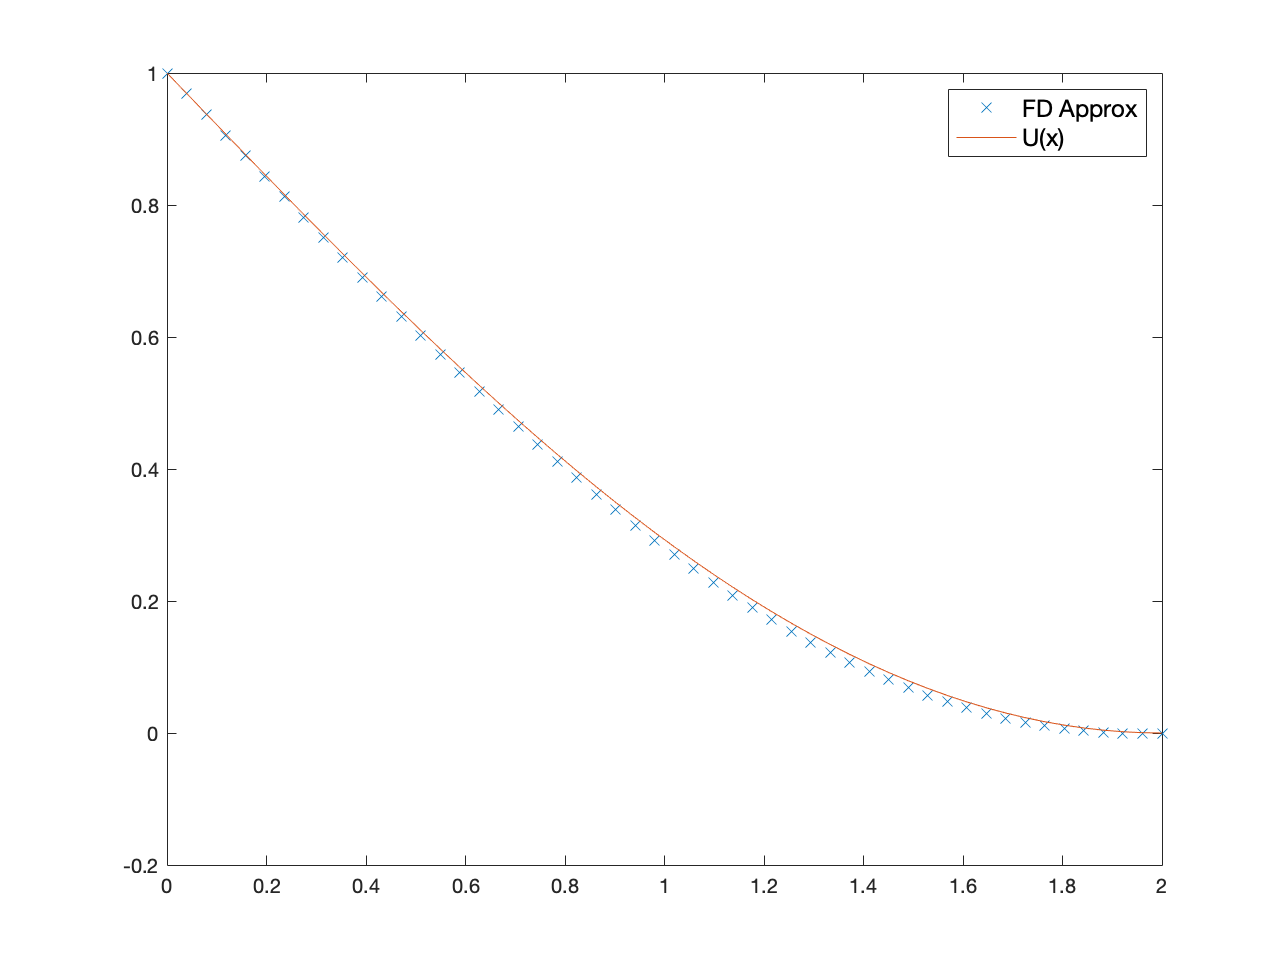
\includegraphics[width=.90\textwidth]{fig.png}
      \end{center}
    \end{figure}


      \textbf{Console:}
      \begin{center}
        \lstinputlisting[basicstyle = \footnotesize]{r10.txt}
      \end{center}
    \item[(c)] Your part (a) code sets up and solves a linear system $AU = F$. For what $q$ values is 
    $A$ strictly diagonally dominant(SDD)?
    \begin{proof} Recall that the matrix $A$ has the form, 
      \begin{equation*}
        A = \frac{1}{h^2}
        \begin{bmatrix}
             (qh^2 - 2) &    1    &         &         &         &         \\ 
                   1 & (qh^2 - 2) &    1    &         &         &         \\ 
                     &    1    & (qh^2 - 2) &    1    &         &         \\ 
                     &         &  \ddots &  \ddots & \ddots  &         \\
                     &         &         &    1    & (qh^2 - 2) &   1     \\
                     &         &         &         &    1    & (qh^2 - 2) 
        \end{bmatrix}.
      \end{equation*}
      To be strictly diagonally dominant for all $i$
      \begin{equation*}
        |a_{ii}|>\sum_{j \neq i} |a_{ij}|.
      \end{equation*}
      Therefore it follows that $A$ is SDD when $|qh^2 - 2| > 2$ and thus either $q > 4/h^2$ or $q < 0$.
    \end{proof}

    \item[(d)] Duplicate the code from part (a), give it a new name bvpqgs(), and implement Gauss-Seidel to 
    solve the linear system, instead of calling the built-in linear solver. Use the problem given in part (b)
    and for each of $m = 5$ and $m = 50$ find nonzero values $q$ where Gauss-Seidel does converge and does not converge. 
    When convergence happens, how many iterations give 8 digit accuracy?
    \solution Recall that SDD is a sufficient condition for Gauss-Seidel iteration to converge. Therefore by part (c) for the problem described in 
    part (a) we know that for $m = 5$ GS iteration will converge if, 
    \begin{equation*}
      q > 16 \qquad q < 0.
    \end{equation*}
    and we know that for $m = 50$, GS iteration will converge if, 
    \begin{equation*}
      q > 49^2 \qquad q < 0.
    \end{equation*}
    Now consider the following matlab code bvpqgs() which replaces the backslash operator with a Gauss-Seidel iteration sub-routine to solve the linear system,\\

    \textbf{Code:}
    \begin{center}
      \lstinputlisting[basicstyle = \footnotesize]{r11.txt}
    \end{center}

    First we will show that for the indicated values of $q$, the problem from part (b) does converge. The following console output 
    shows convergence of $m = 5$ with $q = 20$ within $N = 14$ iterations,\\

    \textbf{Console:}
    \begin{center}
      \lstinputlisting[basicstyle = \tiny]{r12.txt}
    \end{center}


    The following console output shows convergence of $m = 50$ with $q = -1 < 0$, I couldn't figure out the best way to find exactly the number 
    of iterations $N$ and I also played around with measuring absolute or relative error hence the $q = -1$. In doing that I saw the relationship
    explained by $A\hat{U} = F + \tau$ and how convergence in solving the system (increasing $N$) does not mean convergence to the true solution (increasing $m$)
    because of the LTE. The following shows clear convergence within 5000 iterations. 

    \textbf{Console:}
    \begin{center}
      \lstinputlisting[basicstyle = \footnotesize]{r13.txt}
    \end{center}

    Plugging in $m = 5$ and $q = 10$ results in a system which is not SDD, and also does not converge through GS iteration. With $m = 50$ using $q = 1000$ has the same result.\\ 

    \textbf{Console:}
    \begin{center}
      \lstinputlisting[basicstyle = \footnotesize]{r14.txt}
    \end{center}    
  \end{enumerate}
  
\end{exercise}



\begin{exercise}{Problem P16} In calculus you probably learned Newton's method as a memorized formula:
  $x_{k+1} = x_k - f(x_k)/f'(x_k)$. Rewrite equations Newtons's method equations (8), (9) from the slides, 
  in the one-dimensional case, to derive this memorized formula.
  \begin{proof} Recall equations (8) and (9) from class which demonstrate the 'solving a linear system' approach 
    to Newton's method, where $J(x)$ is the evaluation of the jacobian and $f(x)$ is a vector valued function, 
    \begin{equation*}
      J(x_k)s = -f(x_k).
    \end{equation*}
    \begin{equation*}
      x_{k+1} = x_k + s.
    \end{equation*}
    In the one-dimensional case $f(x)$ is no longer a vector valued function and it follows that $J(x_k) = f'(x_k)$. 
    By substitution we simply get $f'(x_k)s = -f(x_k)$, since all our elements are scalars we can divide across to get 
    $s = -f(x_k)/f'(x_k)$. By substitution into equation (9) we get the desired result. 
  \end{proof}
  
\end{exercise}
\vspace{1in}



\begin{exercise}{Problem P17} This problem was assigned in Homework \#2 of Numerical Linear Algebra last Fall. 
  \begin{enumerate}
    \item[(a)] Consider these 3 equations, chosen for visualizability:
    \begin{equation*}
      x^2 + y^2 + z^2 = 4, \qquad x = \cos(\pi x), \qquad z = y^2
    \end{equation*}
    Sketch the surface of each equation in $\RR^3$. Describe informally why there are 
    two solutions of this system of three equations, that is, two points $(x, y, z) \in \RR^3$
    at which all three equations are satisfied. Explain why both solutions are inside the box $-1 \leq x \leq 1, -2 \leq y \leq 2, 0 \leq z \leq 2$.
    \solution Here is a sketch of the three proposed surfaces
    \begin{figure}[H]
      \begin{center}
        \caption{  $x^2 + y^2 + z^2 = 4, \qquad x = \cos(\pi x), \qquad z = y^2$ }
        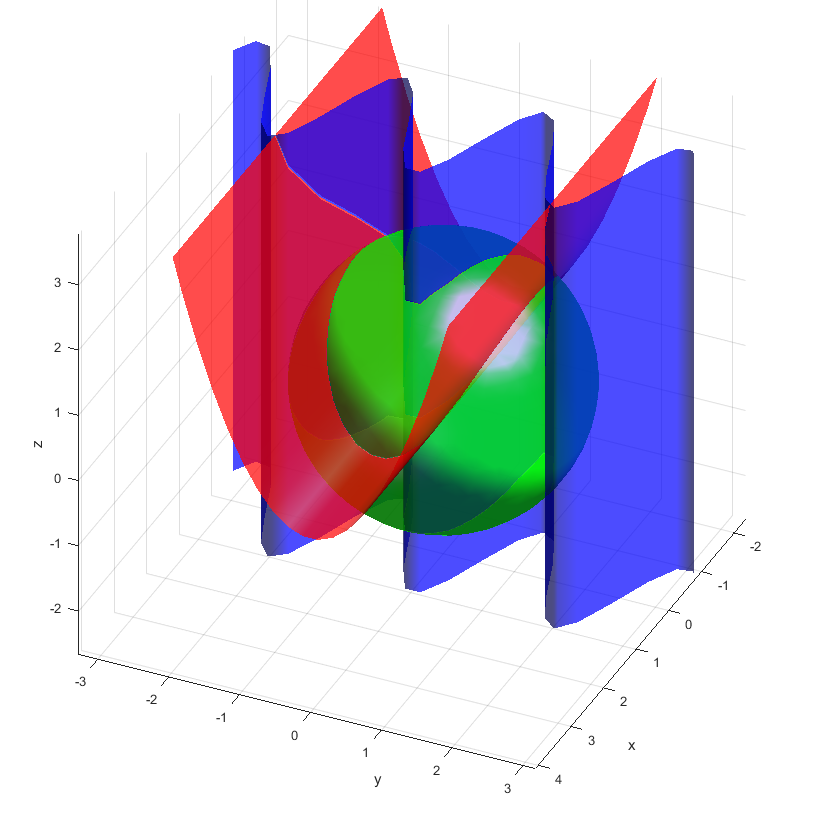
\includegraphics[width=.75\textwidth]{fig2.png}
      \end{center}
    \end{figure}

    \textbf{Code:}
    \begin{center}
      \lstinputlisting[basicstyle = \footnotesize]{firstplot.txt}
    \end{center}

    Describing the solutions we can see that the ellipsoid and the parabolic cylinder intersect at a curve.
    When this curve is projected to the $x-y$ plane it only intersects the function $x = \cos(\pi y)$ in two places. The solutions lie within $-1\leq x \leq 1$ because we are bounded by $x = cos(\pi y)$,
    $0\leq z$ because we are bounded by $z = y^2$, and $-2\leq y \leq 2$ and $z \leq 2$ because we are bounded by $x^2 + y^2 + z^2 = 4$.


    \item[(b)] The slides describe Newton's method for nonlinear systems. Implement it in Matlab to solve the 
    above linear system. Show your script and generate at least five iterations. Use $x_0 = (-1, 1, 1)$ as an initial iterate
    to find one solution, and also find the other solution using a different initial iterate. Note format long is appropriate here. 
    \solution The following is an implementation of Newton's method for solving this system. It abstracts the Jacobian and solves for the 
    derivatives symbolically so one could plug in any 3 equations in $\RR^3$ and attempt to solve the system. \\
    
    \textbf{Code:}
    \begin{center}
      \lstinputlisting[basicstyle = \footnotesize]{r15.txt}
    \end{center}

    The following is the console output for running this routine with an initial iterate $x_0$ generating 6 Newton iterations and also finding the other solution 
    by using $x_0 = (-1, -1, 1)$.\\


    \textbf{Console:}
    \begin{center}
      \lstinputlisting[basicstyle = \footnotesize]{r16.txt}
    \end{center}   






  \end{enumerate}
  
\end{exercise}











\begin{thebibliography}{1}  % "2" because there are two references
  \bibitem{1}
  Iterative Methods for Solving Ax = b—Gauss-Seidel Method | Mathematical Association of America. (n.d.). Retrieved February 19, 2023, from \href{https://www.maa.org/press/periodicals/loci/joma/iterative-methods-for-solving-iaxi-ibi-gauss-seidel-method}{https://www.maa.org/press/periodicals/loci/joma/iterative-methods-for-solving-iaxi-ibi-gauss-seidel-method}
  \bibitem{2}
  Iterative Methods for Solving Ax = b—Jacobi’s Method | Mathematical Association of America. (n.d.). Retrieved February 19, 2023, from \href{https://www.maa.org/press/periodicals/loci/joma/iterative-methods-for-solving-iaxi-ibi-jacobis-method}{https://www.maa.org/press/periodicals/loci/joma/iterative-methods-for-solving-iaxi-ibi-jacobis-method}
  \end{thebibliography}
\end{document}











 




